\documentclass[10pt, a4paper]{article}

\usepackage{ctex}
\usepackage{xeCJK}
\usepackage{caption}
\usepackage{geometry}
\geometry{
    left = 0.6in,
    right = 0.6in,
    top = 0.8in,
    bottom = 1.0in
}
\usepackage{amssymb}
\usepackage{amsbsy}
\usepackage{amsmath}
\usepackage{xcolor}
\usepackage{mathrsfs}
\usepackage{graphicx}
\usepackage{pifont}
\usepackage{tasks}
\settasks{
    label = \Alph*. ,
    label-width = 16pt
}
\pagestyle{empty}

\newcommand{\Title}[3]{
    \begin{center}
        \Large \textbf{中国电子学会 #1~年~#2~月 Scratch~#3级考试}
    \end{center}
}
\newcommand{\TimeAndName}[1]{
    \begin{center}
        考试时间:~#1~ 分钟 \qquad\qquad\qquad\qquad 姓名:\underline{\quad\quad\quad\quad}
    \end{center}
}

\begin{document}
    \Title{2020}{6}{二} % 标题
    \TimeAndName{60} % 考试时间及姓名

    % 单选题
    \vspace{2mm}
    {\noindent\textbf{第一部分、单选题(共 25 题,每题 2 分,共50分.)}}
    \begin{enumerate}
        % 1
        \item 如下图所示脚本运行的结果是?(\qquad)
        \begin{tasks}(4)
            \task 画一条直线
            \task 画一个三角形
            \task 画一个圆形
            \task 画一条虚线
        \end{tasks}

        % 2
        \item 运行如下图所示脚本,下面选项中说法错误的是?(\qquad)
        \begin{tasks}(4)
            \task “笔的颜色”为0
            \task “笔的饱和度”为50
            \task “笔的粗细”为20
            \task “笔的亮度”为20
        \end{tasks}

        % 3
        \item 三个小朋友比年龄大小。根据下面三句话,判断他们中年龄最大的是?(\qquad)
        
        \ding{172}~小芳比小明大2岁;\quad \ding{173}~小燕比小芳小1岁;\quad \ding{174}~小燕比小明大1岁。
        \begin{tasks}(4)
            \task 小芳
            \task 小燕
            \task 小明
            \task 小红
        \end{tasks}

        \begin{figure}[htbp]
            \centering
            \begin{minipage}[t]{.09\textwidth}
                \centering
                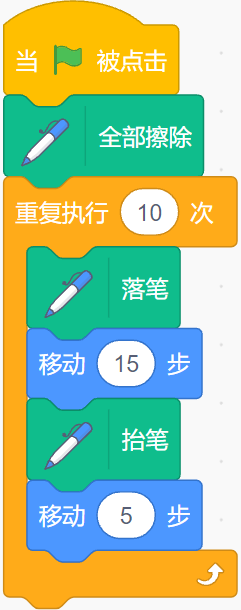
\includegraphics[width=1\textwidth]{1.png}
                \caption*{第1题}
            \end{minipage}
            \begin{minipage}[t]{.17\textwidth}
                \centering
                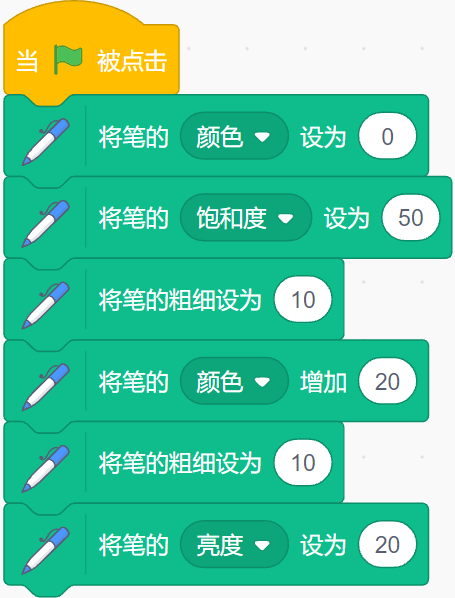
\includegraphics[width=\textwidth]{2.png}
                \caption*{第2题}
            \end{minipage}
            \begin{minipage}[t]{.2\textwidth}
                \centering
                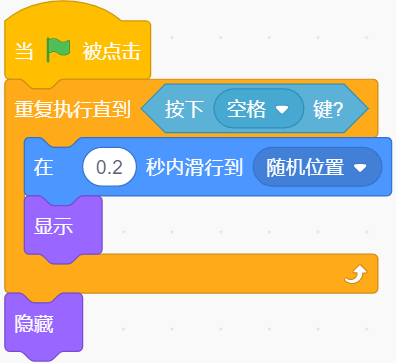
\includegraphics[width=\textwidth]{4.png}
                \caption*{第4题}
            \end{minipage}
            \begin{minipage}[t]{.2\textwidth}
                \centering
                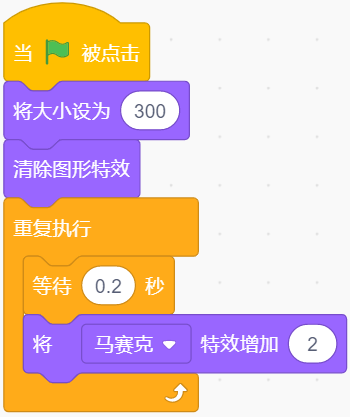
\includegraphics[width=\textwidth]{7.png}
                \caption*{第7题}
            \end{minipage}
            \begin{minipage}[t]{.2\textwidth}
                \centering
                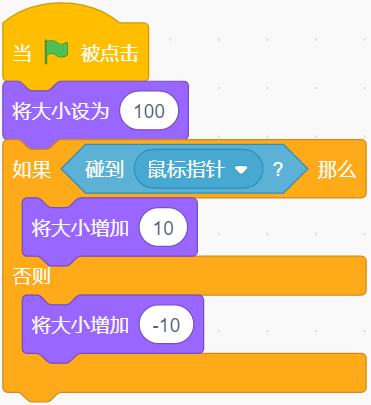
\includegraphics[width=\textwidth]{8.png}
                \caption*{第8题}
            \end{minipage}
        \end{figure}

        % 4
        \item 对于默认的小猫角色,运行如上图所示脚本当按时什么时,角色小猫会隐藏?(\qquad)
        \begin{tasks}(4)
            \task 按下鼠标
            \task 碰到红颜色
            \task 按下空格键
            \task 碰到舞台边缘
        \end{tasks}

        % 5
        \item 运行下面脚本,角色完成什么动作?(\qquad)
        
        \begin{minipage}{.2\textwidth}
            \centering
            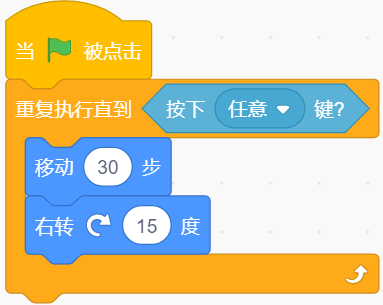
\includegraphics[width=\textwidth]{5.png}
        \end{minipage}
        \begin{minipage}{.68\textwidth}
            \begin{tasks}
                \task 角色向前移动30,然后向右转15度,停止
                \task 角色向前移动30,然后向右转15度,重复执行,画一个圆。
                \task 角色向前移动30,然后向右转15度,重复执行,永不停止。
                \task 角色向前移动30,然后向右转15度,重复执行,直到按下任意键。
            \end{tasks}
        \end{minipage}

        % 6
        \item 在舞台上,小猫从坐标$(90,56)$开始,先向左移动80步,再向上移动24步,此时小猫的坐标是?(\qquad)
        \begin{tasks}(4)
            \task $(10,80)$
            \task $(170,80)$
            \task $(-10,80)$
            \task $(-170,80)$
        \end{tasks}

        % 7
        \item 对于默认的小猫角色,运行如上图所示脚本,舞台上小猫会出现什么?(\qquad)
        \begin{tasks}(4)
            \task 颜色会逐渐改变
            \task 数量会逐渐改变
            \task 颜色会改变一次
            \task 数量会改变一次
        \end{tasks}

        % 8
        \item 运行如上图所示的脚本,角色被点击后的大小是?(\qquad)
        \begin{tasks}(4)
            \task 100
            \task 90
            \task 110
            \task 120
        \end{tasks}

        % 9
        \item 下面坐标哪个可以把角色小猫移动到舞台左下角?(\qquad)
        \begin{tasks}(4)
            \task $x:0,y:0$
            \task $x:170,y:120$
            \task $x:-170,y:-120$
            \task $x:170,y:-120$
        \end{tasks}

        % 10
        \item 运行如下图所示脚本,角色的音量是?(\qquad)
        \begin{tasks}(4)
            \task 39
            \task 40
            \task 49
            \task 50
        \end{tasks}

        % 11
        \item 对于默认的小猫角色,舞台背景如下左图所示,运行如下右图所示脚本小猫最有可能停在舞台的哪里?(\qquad)
        \begin{tasks}(4)
            \task 左上角
            \task 左下角
            \task 右上角
            \task 右下角
        \end{tasks}

        \begin{figure}[htbp]
            \centering
            \begin{minipage}[t]{.18\textwidth}
                \centering
                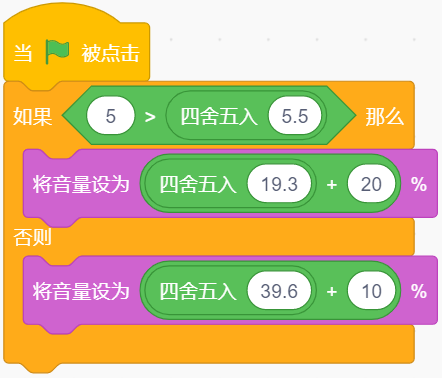
\includegraphics[width=\textwidth]{10.png}
                \caption*{第10题}
            \end{minipage}
            \begin{minipage}[t]{.16\textwidth}
                \centering
                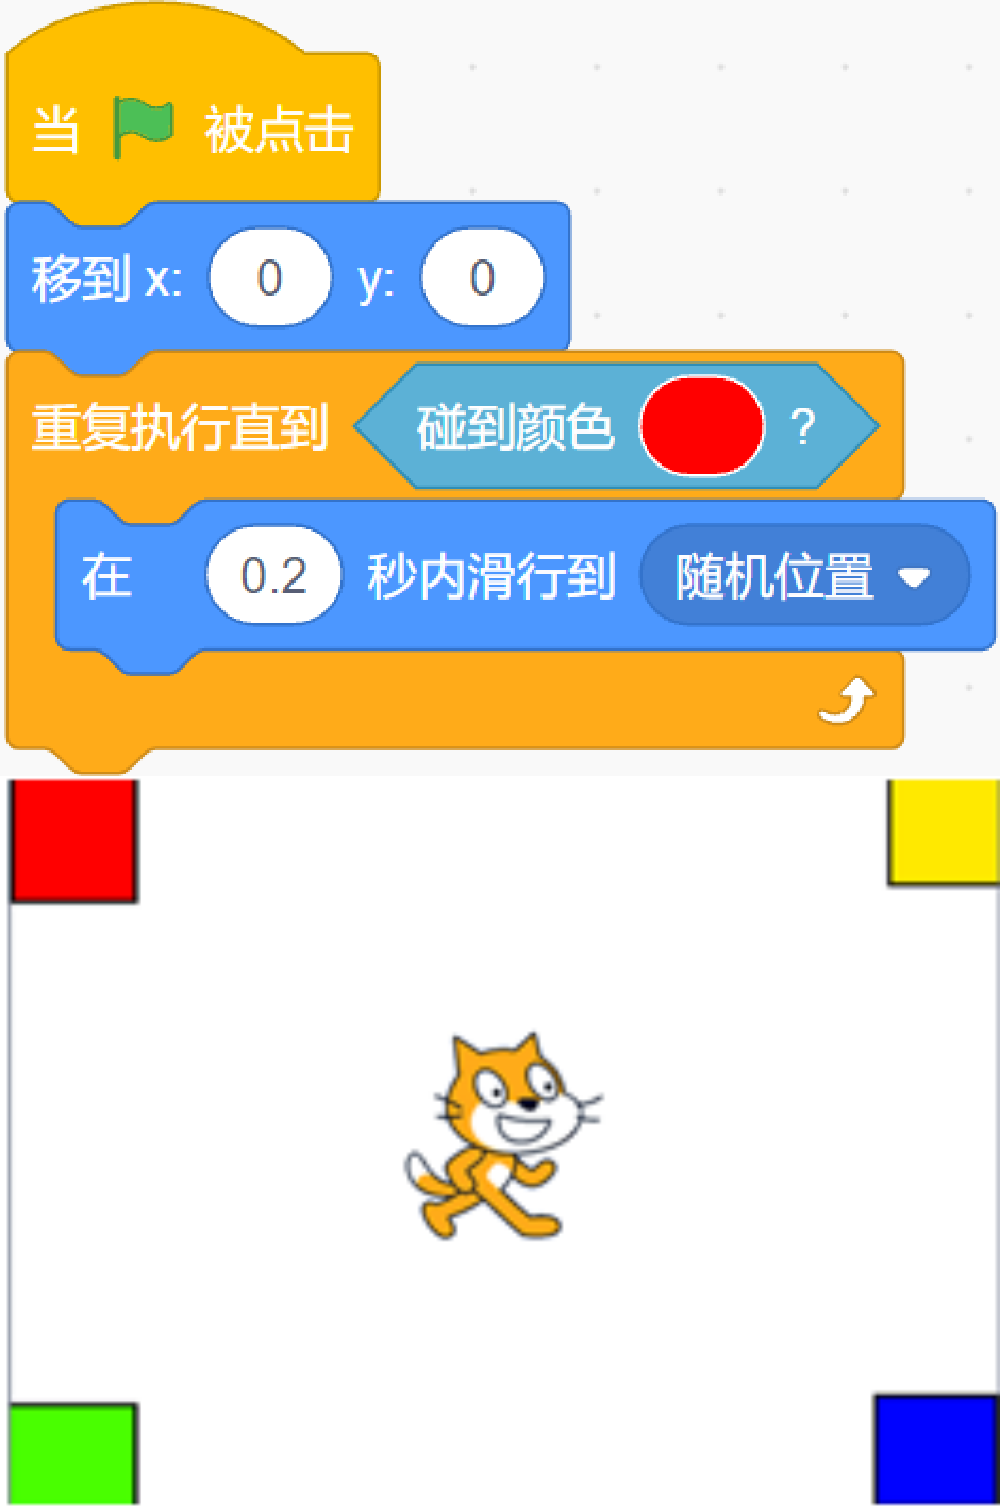
\includegraphics[width=\textwidth]{11.png}
                \caption*{第11题}
            \end{minipage}
            \begin{minipage}[t]{.07\textwidth}
                \centering
                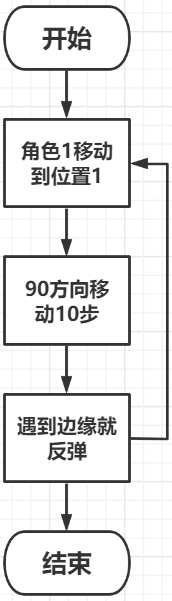
\includegraphics[width=\textwidth]{12.png}
                \caption*{第12题}
            \end{minipage}
            \begin{minipage}[t]{.08\textwidth}
                \centering
                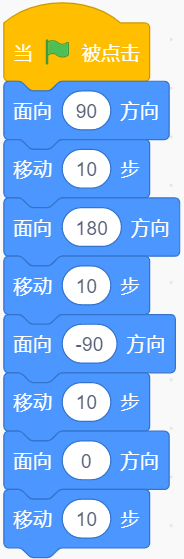
\includegraphics[width=\textwidth]{13.png}
                \caption*{第13题}
            \end{minipage}
            \begin{minipage}[t]{.22\textwidth}
                \centering
                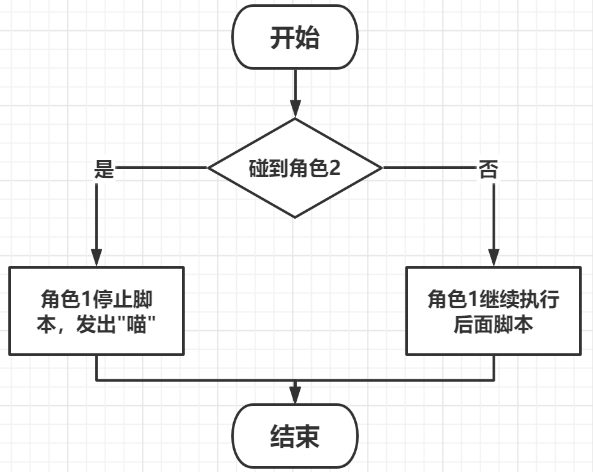
\includegraphics[width=\textwidth]{14.png}
                \caption*{第14题}
            \end{minipage}
            \begin{minipage}[t]{.15\textwidth}
                \centering
                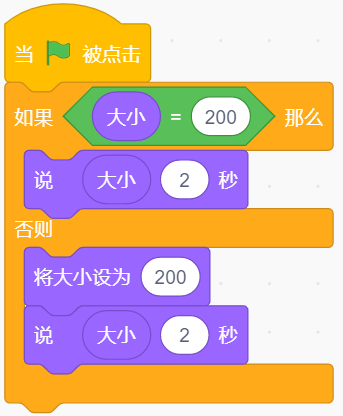
\includegraphics[width=\textwidth]{16.png}
                \caption*{第16题}
            \end{minipage}
            \begin{minipage}[t]{.1\textwidth}
                \centering
                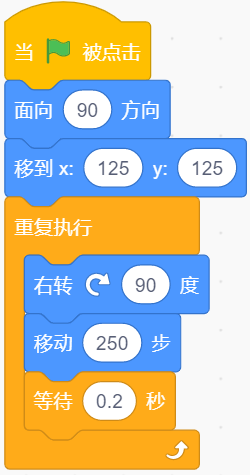
\includegraphics[width=\textwidth]{17.png}
                \caption*{第17题}
            \end{minipage}
        \end{figure}

        % 12
        \item 如上图所示流程图属于什么结构流程图?(\qquad)
        \begin{tasks}(4)
            \task 顺序结构流程图
            \task 循环结构流程图
            \task 选择结构流程图
            \task 语言结构流程图
        \end{tasks}

        % 13
        \item 观察上面脚本,角色初始时面向90度方向,运行脚本后,角色一共改变了几次次方向?(\qquad)
        \begin{tasks}(4)
            \task 2
            \task 3
            \task 4
            \task 5
        \end{tasks}

        % 14
        \item 如上图所示流程图,属于计算机程序结构中的什么?(\qquad)
        \begin{tasks}(4)
            \task 顺序结构
            \task 循环结构
            \task 选择结构
            \task 语言结构
        \end{tasks}
        
        % 15
        \item 在Scratch中坐标$(-100,-100)$在背景舞台的哪个位置?(\qquad)
        \begin{tasks}(4)
            \task 左上角
            \task 右上角
            \task 左下角
            \task 右下角
        \end{tasks}

        % 16
        \item 当角色大小为100时,运行如下图所示脚本,角色说什么2秒?(\qquad)
        \begin{tasks}(4)
            \task 大小
            \task 100
            \task 200
            \task 300
        \end{tasks}

        % 17
        \item 对于默认的小猫角色,运行如下图所示脚本后小猫走出的是?(\qquad)
        \begin{tasks}(4)
            \task 正三角形
            \task 正方形
            \task 正五边形
            \task 正六边形
        \end{tasks}

        % 18
        \item 在以下积木中,哪个可以将声音的音量增大?(\qquad)
        \begin{tasks}(4)
            \task 
\includegraphics[width=.15\textwidth]{18a.png}
            \task 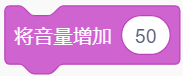
\includegraphics[width=.12\textwidth]{18b.png}
            \task 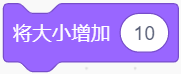
\includegraphics[width=.12\textwidth]{18c.png}
            \task 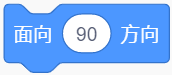
\includegraphics[width=.12\textwidth]{18d.png}
        \end{tasks}

        \newpage
        % 19
        \item 下面哪个积木可以比较两个数字大小?(\qquad)
        \begin{tasks}(4)
            \task 
\includegraphics[width=.1\textwidth]{19a.png}
            \task 
\includegraphics[width=.12\textwidth]{19b.png}
            \task 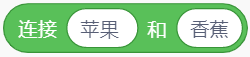
\includegraphics[width=.15\textwidth]{19c.png}
            \task 
\includegraphics[width=.12\textwidth]{19d.png}
        \end{tasks}

        % 20
        \item 运行下面脚本,可以让我们看不到默认小猫?(\qquad)
        \begin{tasks}(4)
            \task 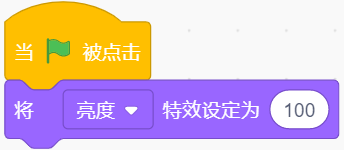
\includegraphics[width=.18\textwidth]{20a.png}
            \task 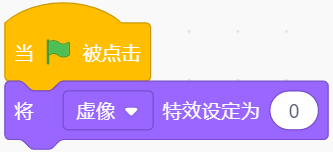
\includegraphics[width=.18\textwidth]{20b.png}
            \task 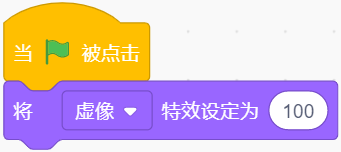
\includegraphics[width=.18\textwidth]{20c.png}
            \task 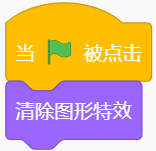
\includegraphics[width=.09\textwidth]{20d.png}
        \end{tasks}

        % 21
        \item 在Scratch中从录制好的声音中截取拷贝出一段声音,你认为最有可能用到下列选项卡中的哪个?(\qquad)
        \begin{tasks}(4)
            \task 
\includegraphics[width=.04\textwidth]{21a.png}
            \task 
\includegraphics[width=.04\textwidth]{21b.png}
            \task 
\includegraphics[width=.04\textwidth]{21c.png}
            \task 
\includegraphics[width=.04\textwidth]{21d.png}
        \end{tasks}

        % 22
        \item 看图找规律,在下图最后一个框中填入什么比较合理?(\qquad)
        \begin{tasks}(4)
            \task 
\includegraphics[width=.05\textwidth]{22a.png}
            \task 
\includegraphics[width=.05\textwidth]{22b.png}
            \task 
\includegraphics[width=.05\textwidth]{22c.png}
            \task 
\includegraphics[width=.05\textwidth]{22d.png}
        \end{tasks}

        % 23
        \item 下面哪个积木可以使舞台中小球碰到舞台边缘反弹?(\qquad)
        \begin{tasks}(4)
            \task 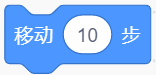
\includegraphics[width=.1\textwidth]{23a.png}
            \task 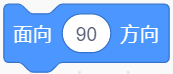
\includegraphics[width=.1\textwidth]{23b.png}
            \task 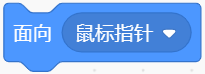
\includegraphics[width=.12\textwidth]{23c.png}
            \task 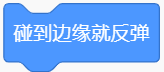
\includegraphics[width=.1\textwidth]{23d.png}
        \end{tasks}

        \begin{figure}[htbp]
            \centering
            \begin{minipage}[t]{.3\textwidth}
                \centering
                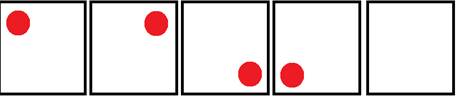
\includegraphics[width=\textwidth]{22.png}
                \caption*{第22题}
            \end{minipage}
            \begin{minipage}[t]{.25\textwidth}
                \centering
                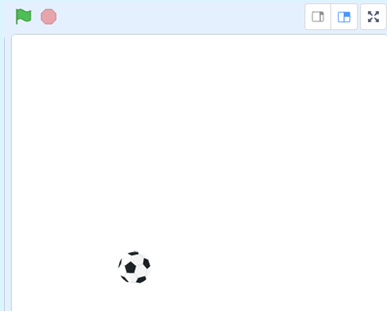
\includegraphics[width=\textwidth]{23.png}
                \caption*{第23题}
            \end{minipage}
            \begin{minipage}[t]{.18\textwidth}
                \centering
                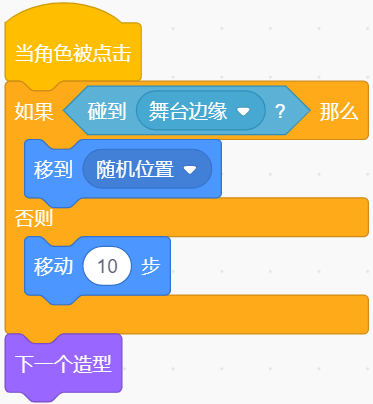
\includegraphics[width=\textwidth]{24.png}
                \caption*{第24题}
            \end{minipage}
        \end{figure}

        % 24
        \item 如上图所示脚本,所对应的流程图应该是?(\qquad)
        \begin{tasks}(4)
            \task 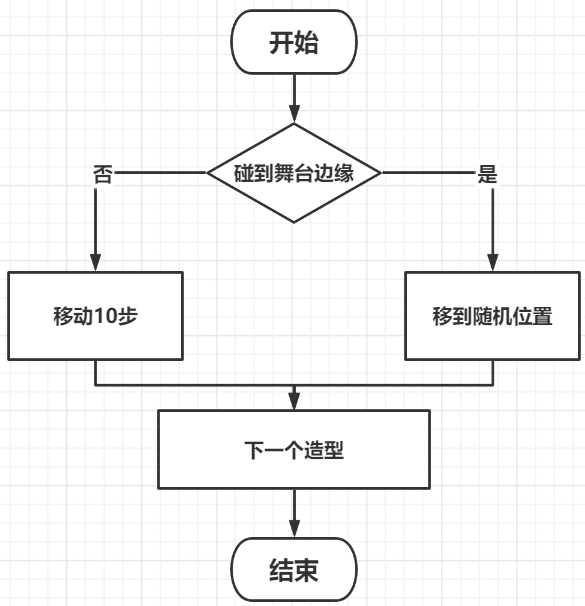
\includegraphics[width=.18\textwidth]{24a.png}
            \task 
\includegraphics[width=.18\textwidth]{24b.png}
            \task 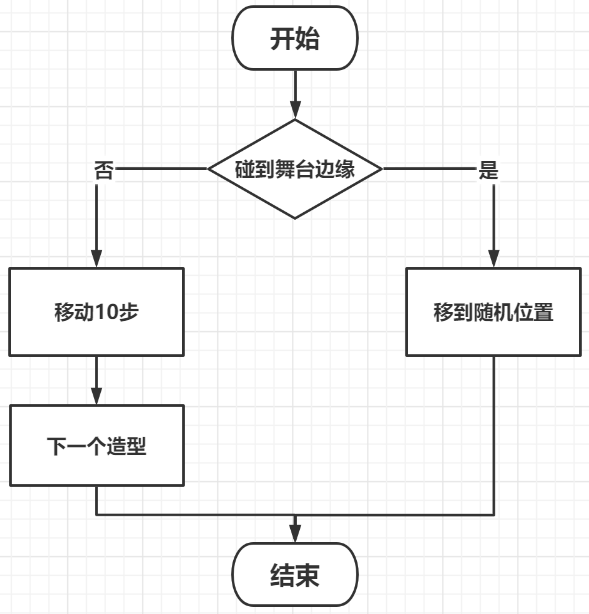
\includegraphics[width=.18\textwidth]{24c.png}
            \task 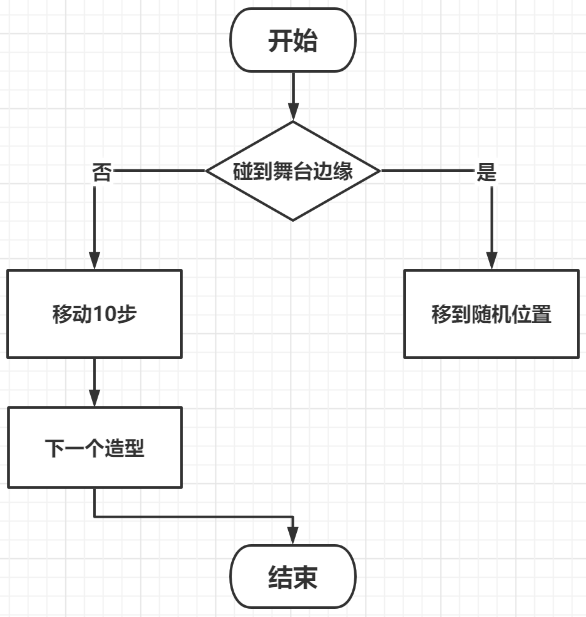
\includegraphics[width=.18\textwidth]{24d.png}
        \end{tasks}
        
        % 25
        \item 运行下列哪个脚本后,默认小猫可以跟随鼠标指针移动?(\qquad)
        \begin{tasks}(4)
            \task 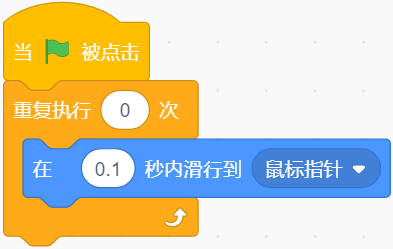
\includegraphics[width=.18\textwidth]{25a.png}
            \task 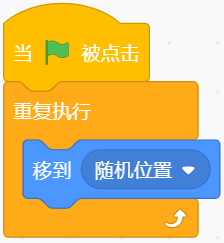
\includegraphics[width=.1\textwidth]{25b.png}
            \task 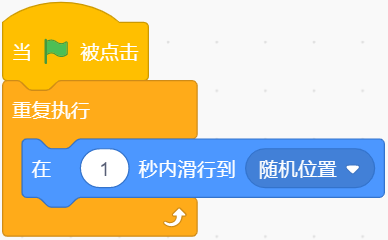
\includegraphics[width=.18\textwidth]{25c.png}
            \task 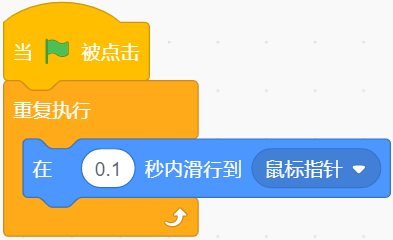
\includegraphics[width=.18\textwidth]{25d.png}
        \end{tasks}
    \end{enumerate}

    \newpage
    % 判断题
    {\noindent\textbf{第二部分、判断题(共 10 题,每题 2 分,共20分.)}}
    \begin{enumerate}
        \setcounter{enumi}{25}
        % 26
        \item 运行如下图所示的脚本,点击绿旗以后,角色将会移动.(\qquad)

        %27
        \item 如图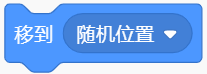
\includegraphics[width=.12\textwidth]{27.png}所示积木,可以让角色在舞台的随机位置出现.(\qquad)
        
        %28
        \item 如图所示
\includegraphics[width=.03\textwidth]{28.png}的按钮中,“\includegraphics[width=.02\textwidth]{28-2.png}”按钮可以在Scratch3中录入声音.(\qquad)
  
        %29
        \item 运行如下图所示的脚本后,可以在舞台上画出一条直线.(\qquad)
        
        %30
        \item 同学们站成一排,从左边数华华是第5人,从右边数第4人是华华,这排共有9人.(\qquad)
        
        %31
        \item 如图\includegraphics[width=.1\textwidth]{31-2.png}所示的“?”处的图形为\includegraphics[width=.02\textwidth]{31-1.png}.(\qquad)
        
        \begin{figure}[htbp]
            \centering
            \begin{minipage}[t]{.24\textwidth}
                \centering
                \includegraphics[width=\textwidth]{26.png}
                \caption*{第26题}
            \end{minipage}
            \begin{minipage}[t]{.12\textwidth}
                \centering
                \includegraphics[width=\textwidth]{29.png}
                \caption*{第29题}
            \end{minipage}
            \begin{minipage}[t]{.11\textwidth}
                \centering
                \includegraphics[width=\textwidth]{32.png}
                \caption*{第32题}
            \end{minipage}
            \begin{minipage}[t]{.14\textwidth}
                \centering
                \includegraphics[width=\textwidth]{33.png}
                \caption*{第33题}
            \end{minipage}
            \begin{minipage}[t]{.16\textwidth}
                \centering
                \includegraphics[width=\textwidth]{34.png}
                \caption*{第34题}
            \end{minipage}
            \begin{minipage}[t]{.11\textwidth}
                \centering
                \includegraphics[width=\textwidth]{35.png}
                \caption*{第35题}
            \end{minipage}
        \end{figure}
        
        %32
        \item 运行如上图所示脚本后,角色的坐标为$(100,100)$.(\qquad)
        
        %33
        \item 运行上图所示的脚本,角色的位置发生了变化.(\qquad)
        
        %34
        \item 运行如上图所示的脚本后,角色碰到颜色“\includegraphics[width=.03\textwidth]{34-2.png}”后会“隐藏”.(\qquad)
        
        %35
        \item 运行如上图所示的脚本,当按下空格键时,角色将增加到150.(\qquad)
    \end{enumerate}

    \newpage
    {\noindent \textbf{第三部分、编程题(共 2 题,共30分.)}}
    \begin{enumerate}
        \setcounter{enumi}{35}
        
        % 36
        \item 别碰红块:
        \begin{figure}[htbp]
            \begin{minipage}{.6\textwidth}
                1. 准备工作
                \begin{tasks}[label = (\arabic*)]
                    \task 导入背景"Blue sky2",删除空白背景;
                    \task 绘制如图红色和绿色正方形颜色块,放在如图所示的大致位置;
                    \task 小猫初始大小为60,初始位置在$(x:-180,y:0)$。
                \end{tasks}
                2. 功能实现
                \begin{tasks}[label = (\arabic*)]
                    \task 通过键盘的“$\uparrow$”、“$\downarrow$”、“$\leftarrow$”、“$\to$”键来控制小猫行走,每按一次,移动4步;
                    \task 小猫在行走过程中需要面向不同方向;
                    \task 当小猫碰到红色时喊出”游戏结束“,并回到初始位置;
                    \task 当小猫碰到绿色时胜利,喊出”胜利!“,并回到初始位置。
                \end{tasks}
            \end{minipage}
            \begin{minipage}{.37\textwidth}
                \centering
                \includegraphics[width=\textwidth]{36.png}
            \end{minipage}
        \end{figure}

        %37
        \item 小鸡捉害虫:
        \begin{figure}[htbp]
            \begin{minipage}{.6\textwidth}
                1. 准备工作
                \begin{tasks}[label = (\arabic*)]
                    \task 删除除小猫;
                    \task 导入背景:“Forest”;
                    \task 导入角色:“Hen”, “Grasshopper”。
                \end{tasks}
                2. 功能实现
                \begin{tasks}[label = (\arabic*)]
                    \task 设置角色:“Hen”初始坐标为$(x=-180,y=-120)$;
                    \task 设置角色:“Grasshopper"初始坐标为随机,角色大小为30;
                    \task 单击绿旗,角色“Hen”向“Grasshopper"移动并留下轨迹;
                    \task 画笔颜色为蓝色,粗细为2;
                    \task 当碰到"Grasshopper"时,母鸡"Hen"发出声音,"Grasshopper"消失。
                \end{tasks}
            \end{minipage}
            \begin{minipage}{.37\textwidth}
                \centering
                \includegraphics[width=\textwidth]{37.png}
            \end{minipage}
        \end{figure}
    \end{enumerate}
\end{document}